\documentclass[letterpaper,twocolumn]{article}

\pdfpagewidth=\paperwidth
\pdfpageheight=\paperheight

%setup double spacing for editing
\usepackage{setspace}
\doublespacing

\usepackage{graphicx} %get graphics commands
\usepackage{times}

\title{Automated Identification and Tracking of Focal Adhesions in Fluorescent TIRF Images}

%get \FloatBarrier command
\usepackage{placeins} 

%give option to use commands like 0.5\textwidth for distances
\usepackage{calc} 
 %allows wraping figures around text
\usepackage{wrapfig}

%adds option to include verbatim input from files
\usepackage{moreverb} 

\begin{document}

\maketitle

\begin{abstract}
text
\end{abstract}

\section*{Introduction}

\section*{Methods}

Several stages are needed to quantitatively examine the FA from a single experiment. Following data collection, the images must be analyzed to locate, track and quantify each focal adhesion.

\subsection*{Image Processing}

[[Image:Cell sample.png|thumb|Results of image processing steps which identify focal adhesions, here outlined in green.]]

In order to first locate and track the FA, sets of images from single experiments were scaled so that the minimum and maximum pixel values in the entire image set were zero and one respectively. The high pass filtration method described previously was to used to find FA in other cell types and has been adapted \cite{Zamir1999}. Briefly, following scaling, each image was filtered with a 25 by 25 pixel averaging filter and the filtered pixel values subtracted from the original pixel values. These image transformations acted as a high pass filter and allowed a single threshold to be used to locate the FA (Figure \ref{cell_sample}). The threshold was determined empirically, but appears to be valid for all experimental data gathered. Between 200 and 400 adhesions were located in each image from the experimental data. With the focal adhesion locations identified in each cell, the properties of the FA were collected including: 

\begin{itemize}
\item size
\item centroid position
\item average pixel value in each adhesion 
\item distance from the cell edge to centroid
\item distance from the cell centroid to centroid
\end{itemize}

\subsection*{FA Tracking and Analysis}

With the focal adhesions identified in each imsage of the experimental data set, another series of algorithms were designed to track the focal adhesions through each sequential image. The tracking algorithm is based on a birth-death model of a FA lifetime. At each time step a FA can either be born, continue into the next time step, merge or die. The birth-death-merge processes are detected by examining the properties extracted from the segmented adhesions. The results of this tracking algorithm are assignments of the individual FA in each image into lineages that track the development of each FA during the course of the experiment.

\begin{figure}[htbp]
\begin{center}
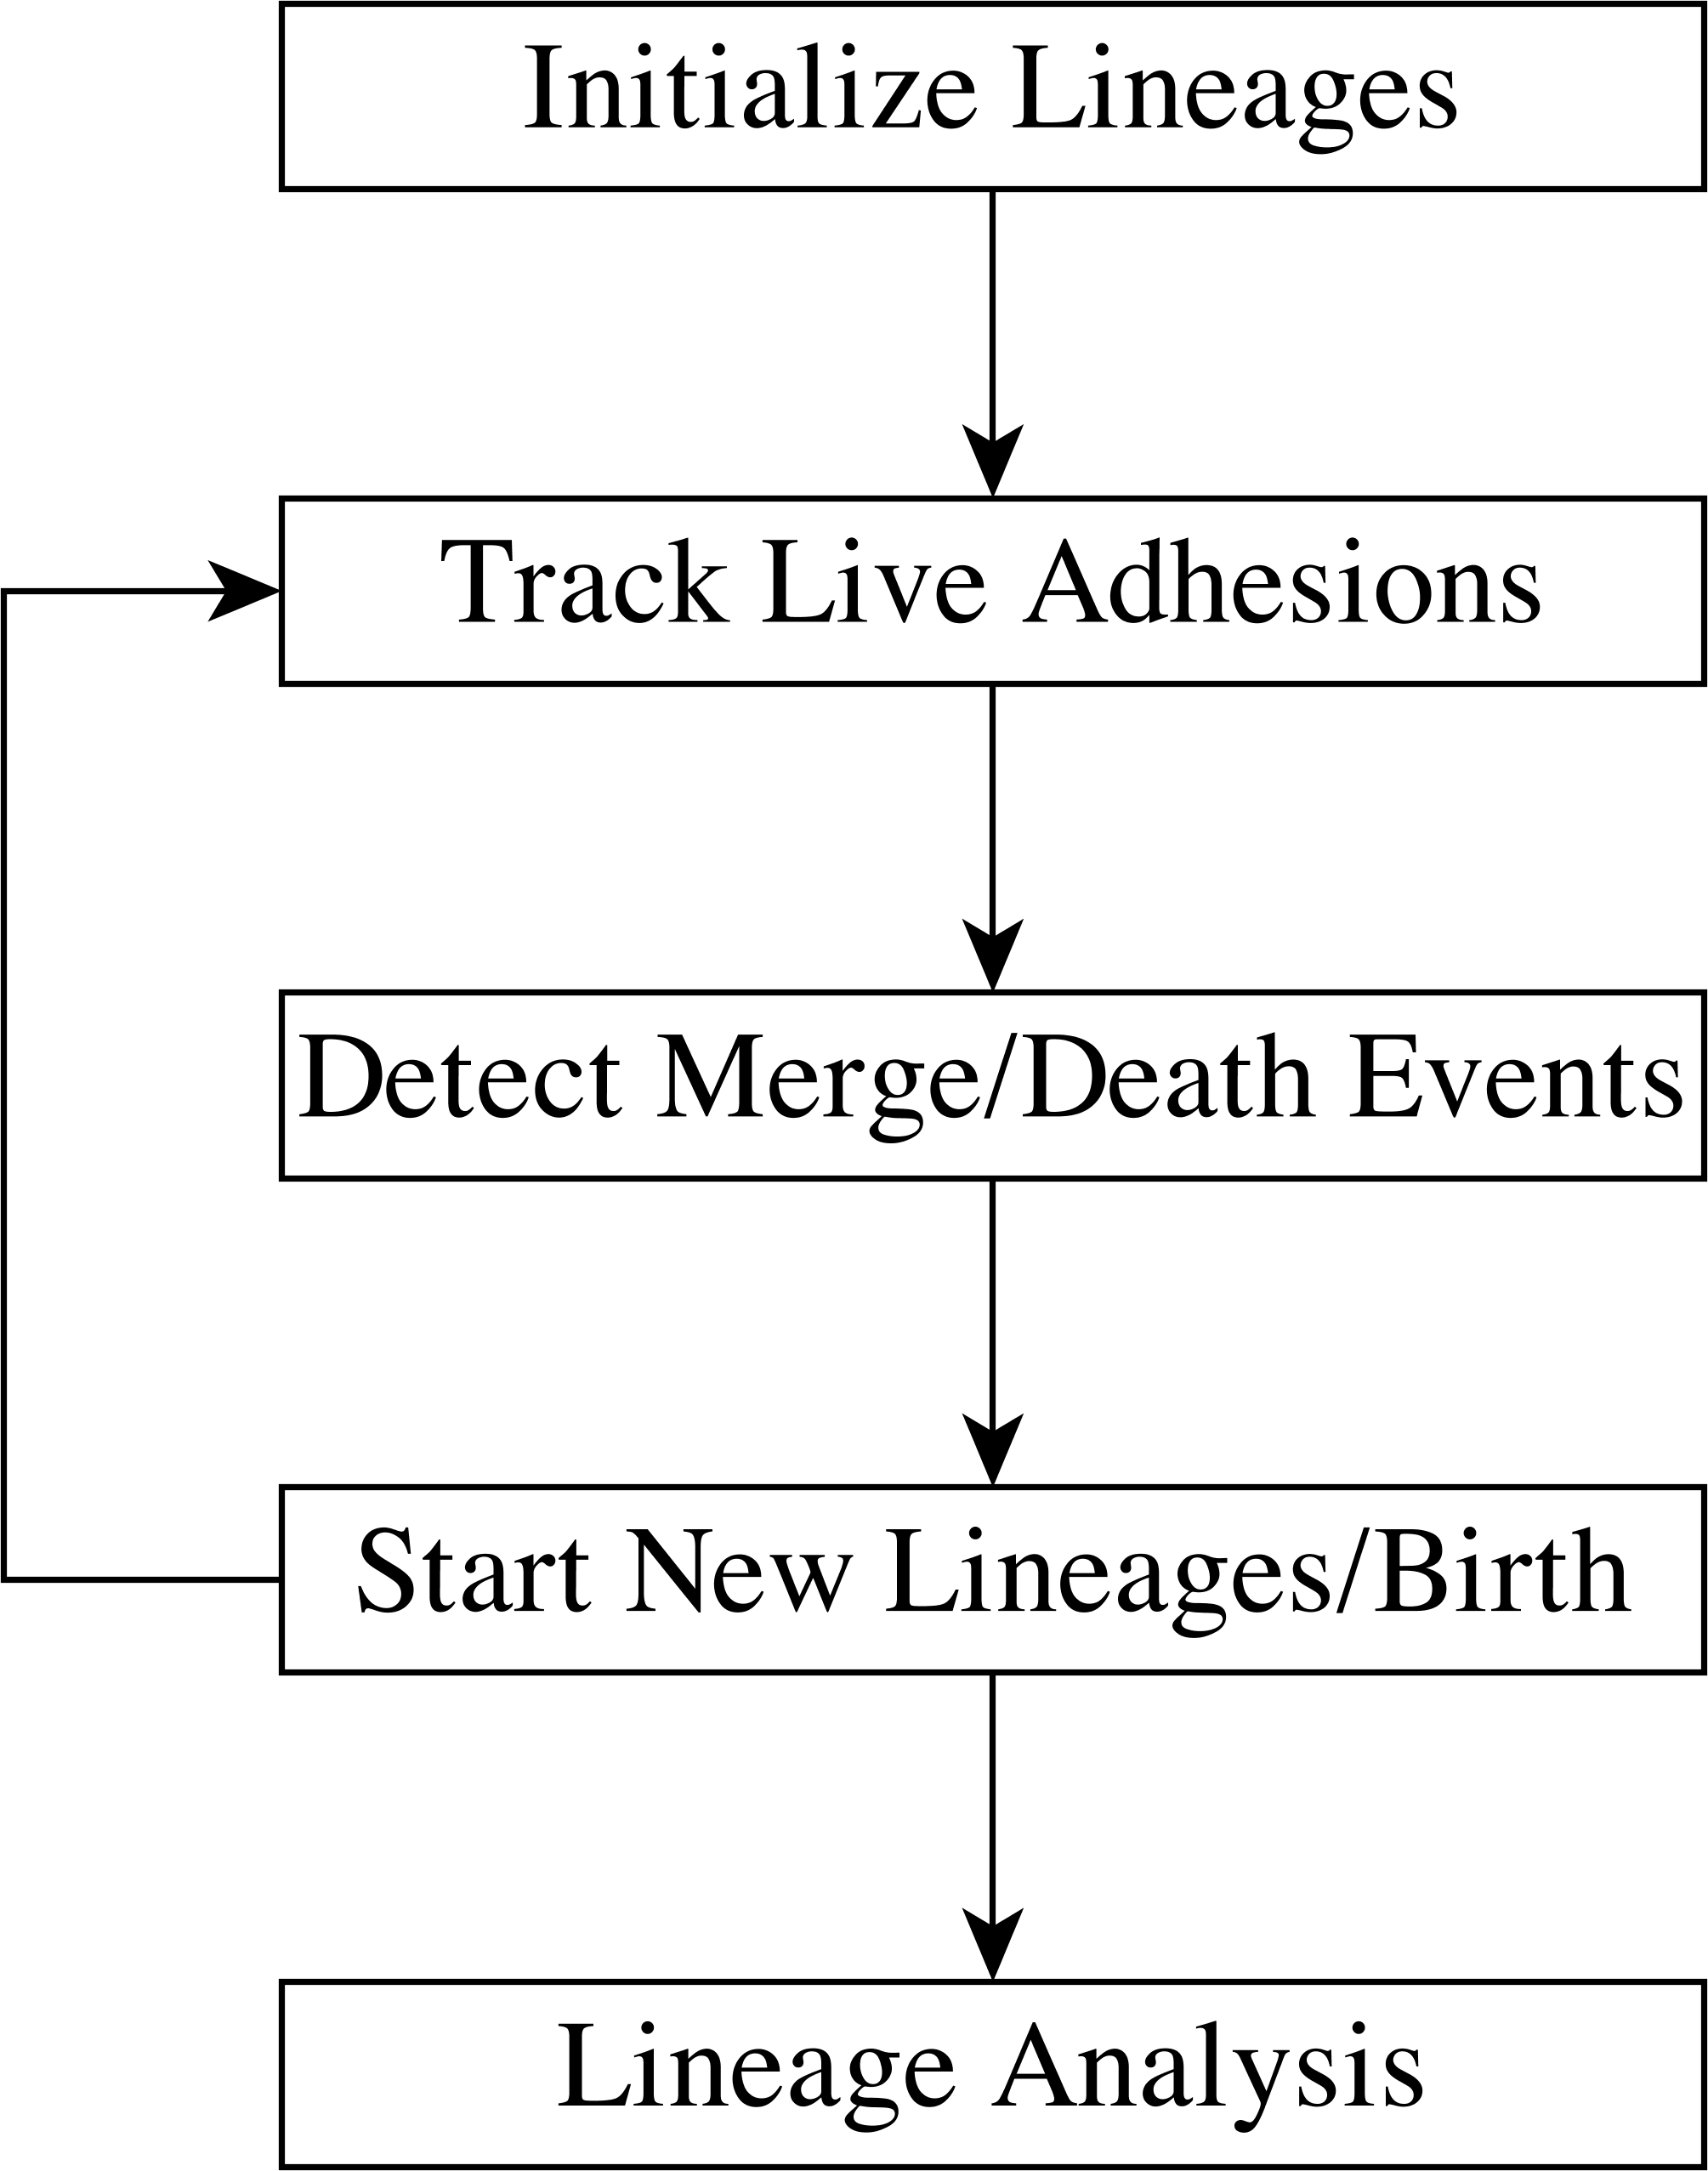
\includegraphics[width=0.5\textwidth]{figures/tracking_chart}
\caption{default}
\label{tracking_chart}
\end{center}
\end{figure}


The tracking algorithm is initialized with all the adhesions detected in the first frame of the image sequence (Figure \ref{tracking_chart}). The first step of the tracking algorithm attempts to locate FA which correspond in the next time step of the experimental data. This first step assumes that if a focal adhesion overlaps with a focal adhesion in the following frame, that these overlapping adhesions correspond to one another. If a FA has no FA which overlap in the following image, the FA closest to that adhesion in terms of the euclidian distance between each adhesion's centroid is assigned as a match. All of the living focal adhesions are assigned a corresponding FA in the following image by these two rules.

This process of assigning live adhesions to corresponding adhesions in the following frame produces sets of adhesions that are predicted to merge. Some of these merge events are true merge events where one adhesion has joined with another, while others are adhesions which die, but are erroneously assigned as merge events. When a FA does not overlap with the predicted merge FA, this FA is assumed to have died. For each of the remaining predicted merge events, one of the FA lineages predicted to merge is continued, while the other FA lineage is predicted to end. When the adhesions predicted to merge differ in size by at least 10\%, the larger adhesion's lineage is continued. If the merging FA's sizes do not differ by at least 10\%, the lineage whose current centroid is closer to the adhesion centroid in the following image is predicted to continue. In this way, each merge event is resolved so that corresponding focal adhesions are collected.

Following tracking live adhesions and resolving the merge and death events, there remain FA in the following image which are not assigned to any of the current lineages. The unassociated FA are assigned into new lineages. This process of tracking the live adhesions, resolving merge and death events and starting new lineages is repeated for each image in the experimental data sequence.

With the FA lineages collected various properties of the FA lineage can be extracted. These include:

\begin{itemize}
\item average pixel value during lifetime
\item average speed
\item longevity
\end{itemize}

\subsection*{Accumulation and Decay Estimates}

To estimate the rates of Paxillin accumulation and decay during the life cycle of a FA, an automated method to identify the slopes of Paxillin concentration versus time curves was developed. 

\section*{Results}

\section*{Conclusion}

\bibliography{all_literature}{}
\bibliographystyle{plain}

\end{document}